\documentclass[14pt,a4paper]{extarticle}

\usepackage{fontspec}
\usepackage{polyglossia}
\setdefaultlanguage{russian}
\setmainfont{Times New Roman}
\newfontfamily\cyrillicfont[Script=Cyrillic]{Times New Roman}
\newfontfamily\cyrillicfonttt[Script=Cyrillic]{Courier New}
\usepackage{amsmath,amssymb}
\usepackage{graphicx}
\usepackage{booktabs}
\usepackage{array}
\usepackage{float}
\usepackage{caption}
\usepackage{enumitem}
\usepackage{geometry}
\usepackage{setspace}
\usepackage{indentfirst}
\usepackage{fancyhdr}
\usepackage{titlesec}
\usepackage[hidelinks]{hyperref}
\hypersetup{
  pdftitle={УИР 1. Статистический анализ результатов измерений},
  pdfauthor={Якименко Владислав Игоревич},
  pdfsubject={Моделирование, вариант 16}
}

\geometry{left=30mm,right=15mm,top=20mm,bottom=20mm}
\setstretch{1.15}
\setlength{\parindent}{1.25cm}
\setlength{\parskip}{0pt}
\captionsetup{labelsep=endash,font=small,justification=centering}
\titleformat{\section}{\bfseries\normalsize}{\thesection.}{0.5em}{}
\titleformat{\subsection}{\bfseries\normalsize}{\thesubsection.}{0.5em}{}
\titlespacing*{\section}{0pt}{1.2ex}{0.8ex}
\titlespacing*{\subsection}{0pt}{1ex}{0.6ex}
\pagestyle{fancy}
\fancyhf{}
\fancyfoot[C]{\thepage}
\renewcommand{\headrulewidth}{0pt}
\setlist[enumerate]{leftmargin=1.25cm,itemsep=0.15em,topsep=0.35em}

\begin{document}

\begin{titlepage}
\begin{center}
Федеральное государственное автономное образовательное учреждение высшего образования\\
«Национальный исследовательский университет ИТМО»\\[0.5cm]
Факультет программной инженерии и компьютерной техники

\vfill

{\bfseries Учебно-исследовательская работа № 1}\\[0.35cm]
{\bfseries «Обработка результатов измерений: статистический анализ числовой последовательности»}\\[0.35cm]
по дисциплине «Моделирование»\\[0.25cm]
Вариант 16

\vfill

\begin{flushright}
\begin{tabular}{ll}
Выполнил: & Якименко Владислав Игоревич \\
Группа: & P3313 \\
Проверил: & Авксентьева Елена Юрьевна
\end{tabular}
\end{flushright}

\vfill

Санкт-Петербург\\
2026
\end{center}
\end{titlepage}

\tableofcontents
\newpage

\section{Цель работы и исходные данные}

Цель работы --- изучить методы статистической обработки результатов измерений: оценить числовые характеристики заданной последовательности, исследовать её случайность и зависимость наблюдений, подобрать аппроксимирующий закон распределения по двум начальным моментам, реализовать генератор и сравнить сгенерированную последовательность с исходной.

В работе используется вариант 16: 300 неотрицательных значений. Расчёты выполняются для объёмов выборки $n=10,20,50,100,200,300$. В качестве эталонных для исходной последовательности принимаются характеристики, рассчитанные при $n=300$.

\begin{figure}[H]
\centering
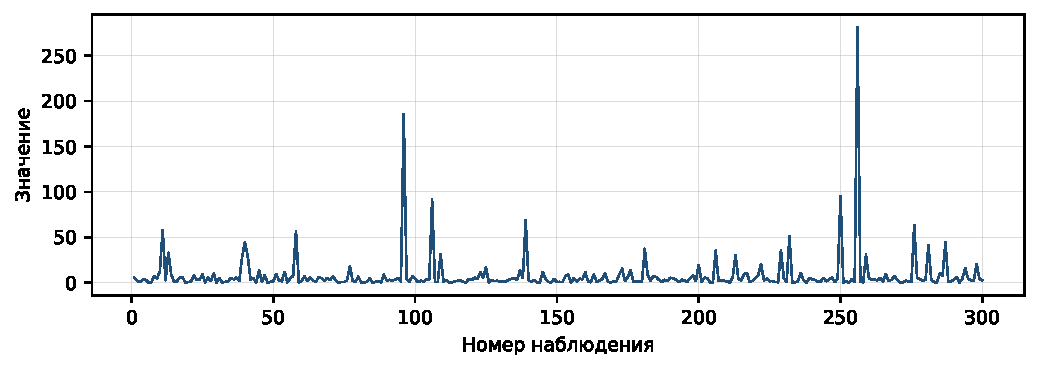
\includegraphics[width=0.93\textwidth]{figures/source_sequence.pdf}
\caption{Значения исходной числовой последовательности}
\end{figure}

\textbf{Вывод.} Последовательность не является монотонной. На графике нет устойчивого тренда и выраженной периодичности. Большая часть значений сосредоточена вблизи нуля, однако присутствуют отдельные крупные наблюдения, что указывает на распределение с длинным правым хвостом.

\section{Числовые характеристики исходной последовательности}

\subsection{Расчётные формулы}

Для первых $n$ наблюдений выборочное среднее рассчитывается по формуле
\begin{equation}
\bar{x}_n=\frac{1}{n}\sum_{i=1}^{n}x_i.
\end{equation}

Несмещённая выборочная дисперсия, среднеквадратическое отклонение и коэффициент вариации определяются выражениями
\begin{equation}
s_n^2=\frac{1}{n-1}\sum_{i=1}^{n}\left(x_i-\bar{x}_n\right)^2,
\qquad
s_n=\sqrt{s_n^2},
\qquad
C_{v,n}=\frac{s_n}{\bar{x}_n}.
\end{equation}

Для доверительной вероятности $p$ интервал для математического ожидания записывается как
\begin{equation}
I_p=\left[\bar{x}_n-\Delta_p;\,\bar{x}_n+\Delta_p\right],
\qquad
\Delta_p=t_p\frac{s_n}{\sqrt{n}},
\end{equation}
где для вероятностей $0{,}90$, $0{,}95$ и $0{,}99$ приняты значения $t_p=1{,}643$, $1{,}960$ и $2{,}576$ соответственно.

Относительное отклонение характеристики $A_n$ от результата для полной выборки определяется формулой
\begin{equation}
\delta_n(A)=\frac{|A_n-A_{300}|}{|A_{300}|}\cdot100\%.
\end{equation}

\begin{table}[H]
\centering
\caption{Характеристики заданной числовой последовательности}
\scriptsize
\resizebox{\textwidth}{!}{%
\begin{tabular}{lrrrrrr}
\toprule
Характеристика & 10 & 20 & 50 & 100 & 200 & 300 \\
\midrule
Математическое ожидание & 4.0583 & 7.9090 & 7.1905 & 7.7709 & 6.8667 & 8.0208 \\
$\Delta_{0.90}$ & 1.9665 & 5.1030 & 2.7034 & 3.3882 & 1.9695 & 2.1431 \\
$\Delta_{0.95}$ & 2.3460 & 6.0876 & 3.2250 & 4.0420 & 2.3495 & 2.5566 \\
$\Delta_{0.99}$ & 3.0833 & 8.0008 & 4.2385 & 5.3123 & 3.0879 & 3.3601 \\
Дисперсия & 14.3262 & 192.9336 & 135.3663 & 425.2796 & 287.3934 & 510.4309 \\
СКО & 3.7850 & 13.8901 & 11.6347 & 20.6223 & 16.9527 & 22.5927 \\
Коэффициент вариации & 0.9326 & 1.7562 & 1.6181 & 2.6538 & 2.4688 & 2.8168 \\
\bottomrule
\end{tabular}}
\end{table}

\begin{table}[H]
\centering
\caption{Относительные отклонения от значений при $n=300$, \%}
\scriptsize
\resizebox{\textwidth}{!}{%
\begin{tabular}{lrrrrrr}
\toprule
Характеристика & 10 & 20 & 50 & 100 & 200 & 300 \\
\midrule
Математическое ожидание & 49.4 & 1.4 & 10.4 & 3.1 & 14.4 & 0.0 \\
$\Delta_{0.90}$ & 8.2 & 138.1 & 26.1 & 58.1 & 8.1 & 0.0 \\
$\Delta_{0.95}$ & 8.2 & 138.1 & 26.1 & 58.1 & 8.1 & 0.0 \\
$\Delta_{0.99}$ & 8.2 & 138.1 & 26.1 & 58.1 & 8.1 & 0.0 \\
Дисперсия & 97.2 & 62.2 & 73.5 & 16.7 & 43.7 & 0.0 \\
СКО & 83.2 & 38.5 & 48.5 & 8.7 & 25.0 & 0.0 \\
Коэффициент вариации & 66.9 & 37.7 & 42.6 & 5.8 & 12.4 & 0.0 \\
\bottomrule
\end{tabular}}
\end{table}

\textbf{Вывод.} При $n=300$ получены $\bar{x}=8{,}0208$, $s^2=510{,}4309$, $s=22{,}5927$ и $C_v=2{,}8168$. Малые выборки дают нестабильные оценки, особенно дисперсии. Значение $C_v>1$ подтверждает высокую относительную вариативность и служит основанием для выбора гиперэкспоненциальной модели.

\section{Анализ распределения исходной последовательности}

Диапазон от нуля до максимального наблюдения разбит на $m=15$ равных интервалов. Ширина интервала и его частота вычисляются как
\begin{equation}
h=\frac{x_{\max}-x_{\min}}{m},
\qquad
n_j=\sum_{i=1}^{n}\mathbf{1}\!\left\{x_i\in[a_j,a_j+h)\right\},
\qquad
\widehat{p}_j=\frac{n_j}{n}.
\end{equation}

\begin{figure}[H]
\centering
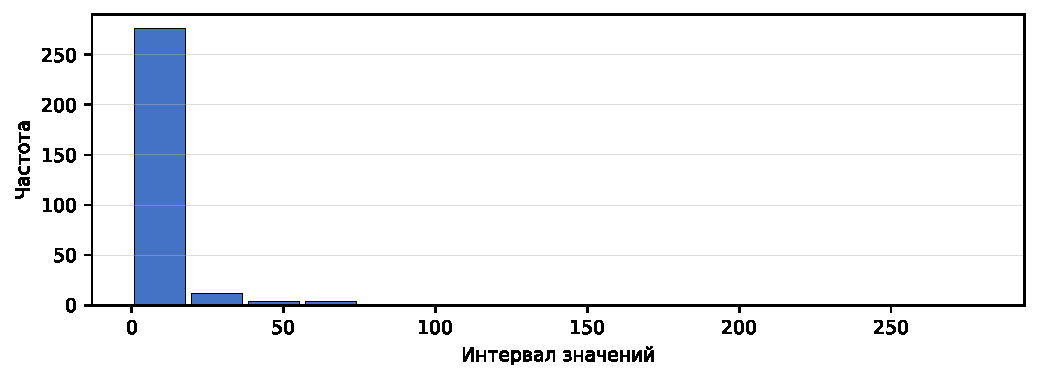
\includegraphics[width=0.93\textwidth]{figures/source_histogram.pdf}
\caption{Гистограмма распределения частот исходной последовательности}
\end{figure}

\textbf{Вывод.} Гистограмма имеет выраженный максимум в первом интервале и длинный правый хвост. Распределение не является симметричным, поэтому нормальная модель для него непригодна. Для дальнейшей аппроксимации нужен неотрицательный закон, допускающий коэффициент вариации больше единицы.

\section{Автокорреляционный анализ исходной последовательности}

Для сдвига $k$ коэффициент автокорреляции рассчитывается как коэффициент корреляции Пирсона между двумя подпоследовательностями длины $n-k$:
\begin{equation}
r_k=
\frac{\displaystyle\sum_{i=1}^{n-k}(x_i-\bar{x}_{1,k})(x_{i+k}-\bar{x}_{2,k})}
{\displaystyle\sqrt{\sum_{i=1}^{n-k}(x_i-\bar{x}_{1,k})^2}
\sqrt{\sum_{i=1}^{n-k}(x_{i+k}-\bar{x}_{2,k})^2}},
\end{equation}
где $\bar{x}_{1,k}$ и $\bar{x}_{2,k}$ --- средние соответствующих подпоследовательностей. Ориентировочная граница значимости на уровне 95\% равна
\begin{equation}
r_{\mathrm{кр}}=\pm\frac{1{,}96}{\sqrt{n}}=\pm0{,}113.
\end{equation}

Для совместной проверки первых $m=10$ коэффициентов используется статистика Льюнга--Бокса
\begin{equation}
Q(m)=n(n+2)\sum_{k=1}^{m}\frac{r_k^2}{n-k}.
\end{equation}

\begin{table}[H]
\centering
\caption{Коэффициенты автокорреляции исходной ЧП}
\small
\resizebox{\textwidth}{!}{%
\begin{tabular}{lrrrrrrrrrr}
\toprule
Сдвиг & 1 & 2 & 3 & 4 & 5 & 6 & 7 & 8 & 9 & 10 \\
\midrule
$r_k$ & -0.041 & -0.039 & 0.034 & -0.040 & -0.045 & 0.135 & -0.029 & -0.057 & -0.027 & 0.082 \\
\bottomrule
\end{tabular}}
\end{table}

\begin{figure}[H]
\centering
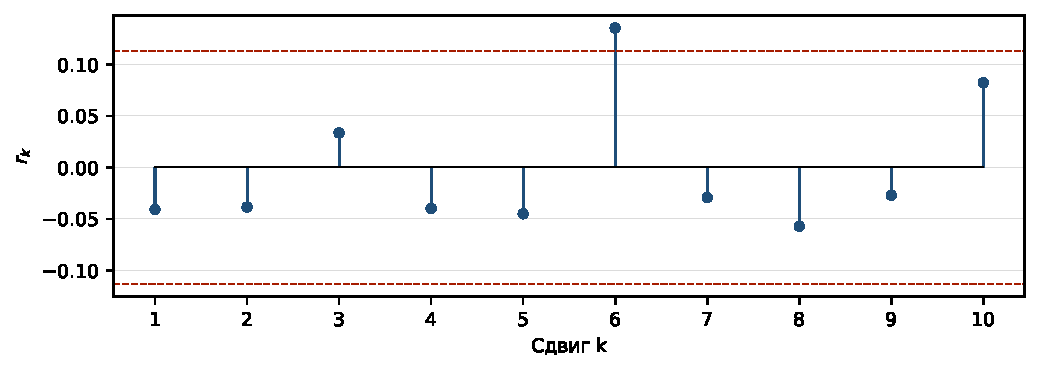
\includegraphics[width=0.93\textwidth]{figures/source_acf.pdf}
\caption{Автокорреляционная функция исходной последовательности}
\end{figure}

Получено $Q(10)=11{,}683$, $p\text{-value}=0{,}307$.

\textbf{Вывод.} Один коэффициент немного выходит за ориентировочную границу, однако совокупный критерий даёт $p\text{-value}>0{,}05$. Оснований отвергать гипотезу об отсутствии серийной зависимости нет.

\section{Аппроксимация закона распределения}

\subsection{Выбор закона}

Для полной выборки $C_v=2{,}8168>1$, поэтому применяется двухфазное гиперэкспоненциальное распределение $H_2$ --- смесь двух экспоненциальных распределений. Его плотность имеет вид
\begin{equation}
f(x)=p\mu_1e^{-\mu_1x}+(1-p)\mu_2e^{-\mu_2x},
\qquad x\geq0.
\end{equation}

Первые два начальных момента и дисперсия модели определяются выражениями
\begin{equation}
\mathbb{E}[X]=\frac{p}{\mu_1}+\frac{1-p}{\mu_2},
\qquad
\mathbb{E}[X^2]=\frac{2p}{\mu_1^2}+\frac{2(1-p)}{\mu_2^2},
\qquad
\mathbb{D}[X]=\mathbb{E}[X^2]-\bigl(\mathbb{E}[X]\bigr)^2.
\end{equation}

\subsection{Параметры распределения $H_2$}

Для согласования первых двух моментов использована сбалансированная параметризация:
\begin{equation}
p=\frac{1}{2}\left(1+\sqrt{\frac{C_v^2-1}{C_v^2+1}}\right),
\qquad
\mu_1=\frac{2p}{\bar{x}},
\qquad
\mu_2=\frac{2(1-p)}{\bar{x}}.
\end{equation}

\begin{table}[H]
\centering
\caption{Параметры распределения $H_2$}
\small
\begin{tabular}{lr}
\toprule
Параметр & Значение \\
\midrule
Вероятность ветви $p$ & 0.940494 \\
Интенсивность $\mu_1$ & 0.234515 \\
Интенсивность $\mu_2$ & 0.014838 \\
\bottomrule
\end{tabular}
\end{table}

Ожидаемое число наблюдений модели в интервале $[a_j,b_j)$ рассчитывается по функции распределения:
\begin{equation}
\widehat{n}_j=n\!\left[
p\left(e^{-\mu_1a_j}-e^{-\mu_1b_j}\right)
+(1-p)\left(e^{-\mu_2a_j}-e^{-\mu_2b_j}\right)
\right].
\end{equation}

\begin{figure}[H]
\centering
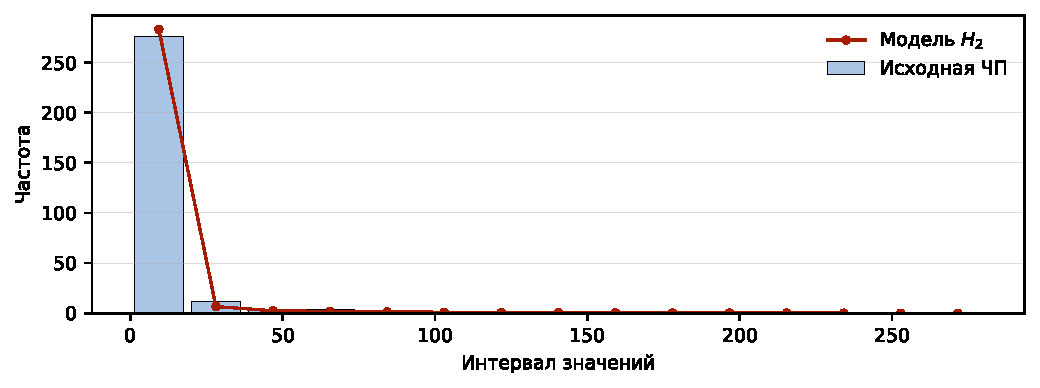
\includegraphics[width=0.93\textwidth]{figures/h2_fit.pdf}
\caption{Сопоставление гистограммы и теоретической модели $H_2$}
\end{figure}

\textbf{Вывод.} Модель $H_2$ воспроизводит основной пик распределения и длинный правый хвост. Аппроксимация по двум моментам согласует математическое ожидание и дисперсию исходной последовательности, но не обязана точно совпадать с каждой интервальной частотой.

\section{Алгоритм генерации случайной последовательности}

Для генерации используются два числа $U_1,U_2\in(0;1)$. Их формирует линейный конгруэнтный генератор с фиксированным начальным состоянием $S_0=8141$:
\begin{equation}
S_{k+1}=\left(1664525S_k+1013904223\right)\bmod 2^{32},
\qquad
U_k=\frac{S_k+0{,}5}{2^{32}}.
\end{equation}

Число $U_1$ выбирает фазу смеси, а $U_2$ преобразуется методом обратной функции распределения:
\begin{equation}
X=
\begin{cases}
-\dfrac{\ln U_2}{\mu_1}, & U_1\leq p,\\[0.8em]
-\dfrac{\ln U_2}{\mu_2}, & U_1>p.
\end{cases}
\end{equation}

Алгоритм реализации:
\begin{enumerate}
\item задать $p$, $\mu_1$, $\mu_2$ и начальное состояние LCG;
\item для каждого наблюдения получить $U_1$ и $U_2$;
\item по $U_1$ выбрать быструю или медленную экспоненциальную ветвь;
\item по $U_2$ вычислить $X$ методом обратного преобразования;
\item повторить шаги до получения 300 значений.
\end{enumerate}

Расчётная формула в Excel:
\begin{equation*}
\texttt{IF(U1<=p; -LN(U2)/mu1; -LN(U2)/mu2)}.
\end{equation*}

\begin{figure}[H]
\centering
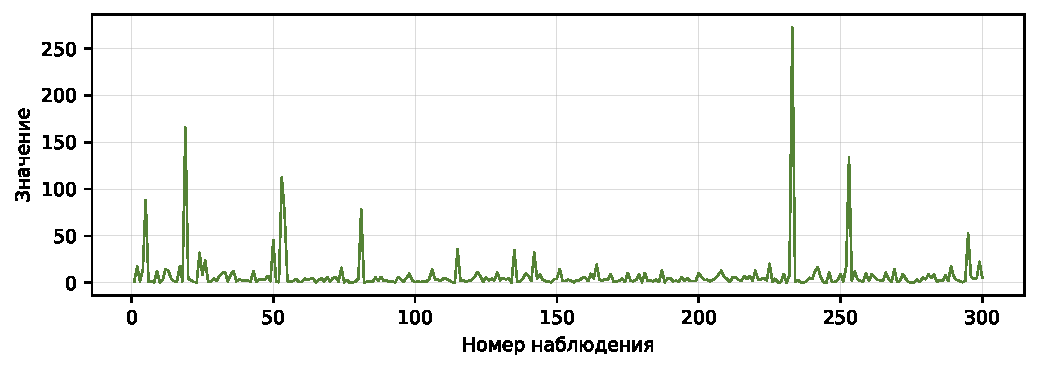
\includegraphics[width=0.76\textwidth]{figures/generated_sequence.pdf}
\caption{Результат работы генератора $H_2$}
\end{figure}

\textbf{Вывод.} Фиксированное начальное состояние делает результат повторяемым. На графике, как и у исходных данных, большинство значений невелико, но встречаются редкие большие выбросы.

\section{Сравнение исходной и сгенерированной последовательностей}

\subsection{Сравнение числовых характеристик}

Для сгенерированного ряда характеристики рассчитаны по формулам (1)--(3). Отклонение от исходной последовательности того же объёма вычисляется как
\begin{equation}
\delta_n^{(\mathrm{ген}/\mathrm{исх})}(A)=
\frac{\left|A_n^{(\mathrm{ген})}-A_n^{(\mathrm{исх})}\right|}
{\left|A_n^{(\mathrm{исх})}\right|}\cdot100\%.
\end{equation}

\begin{table}[H]
\centering
\caption{Характеристики сгенерированной случайной ЧП}
\scriptsize
\resizebox{\textwidth}{!}{%
\begin{tabular}{lrrrrrr}
\toprule
Характеристика & 10 & 20 & 50 & 100 & 200 & 300 \\
\midrule
Математическое ожидание & 13.7252 & 18.1052 & 11.6250 & 9.8000 & 7.3415 & 8.0289 \\
$\Delta_{0.90}$ & 14.0041 & 14.5911 & 6.1499 & 3.9242 & 2.0449 & 2.1422 \\
$\Delta_{0.95}$ & 16.7060 & 17.4063 & 7.3365 & 4.6813 & 2.4395 & 2.5555 \\
$\Delta_{0.99}$ & 21.9565 & 22.8769 & 9.6422 & 6.1526 & 3.2061 & 3.3587 \\
Дисперсия & 726.4951 & 1577.3604 & 700.5429 & 570.4542 & 309.8159 & 509.9885 \\
СКО & 26.9536 & 39.7160 & 26.4678 & 23.8842 & 17.6016 & 22.5829 \\
Коэффициент вариации & 1.9638 & 2.1936 & 2.2768 & 2.4372 & 2.3975 & 2.8127 \\
\bottomrule
\end{tabular}}
\end{table}

\begin{table}[H]
\centering
\caption{Отклонения сгенерированной ЧП от исходной того же объёма, \%}
\scriptsize
\resizebox{\textwidth}{!}{%
\begin{tabular}{lrrrrrr}
\toprule
Характеристика & 10 & 20 & 50 & 100 & 200 & 300 \\
\midrule
Математическое ожидание & 238.2 & 128.9 & 61.7 & 26.1 & 6.9 & 0.1 \\
$\Delta_{0.90}$ & 612.1 & 185.9 & 127.5 & 15.8 & 3.8 & 0.0 \\
$\Delta_{0.95}$ & 612.1 & 185.9 & 127.5 & 15.8 & 3.8 & 0.0 \\
$\Delta_{0.99}$ & 612.1 & 185.9 & 127.5 & 15.8 & 3.8 & 0.0 \\
Дисперсия & 4971.1 & 717.6 & 417.5 & 34.1 & 7.8 & 0.1 \\
СКО & 612.1 & 185.9 & 127.5 & 15.8 & 3.8 & 0.0 \\
Коэффициент вариации & 110.6 & 24.9 & 40.7 & 8.2 & 2.9 & 0.1 \\
\bottomrule
\end{tabular}}
\end{table}

При $n=300$ математическое ожидание сгенерированной последовательности равно $8{,}0289$, дисперсия --- $509{,}9885$. Отклонения от исходных значений составляют $0{,}10\%$ и $0{,}09\%$ соответственно.

\textbf{Вывод.} На полной выборке первые два момента воспроизведены с отклонением менее $0{,}1\%$. Различия на малых объёмах закономерно больше из-за высокой дисперсии распределения.

\subsection{Сравнение распределений}

\begin{figure}[H]
\centering
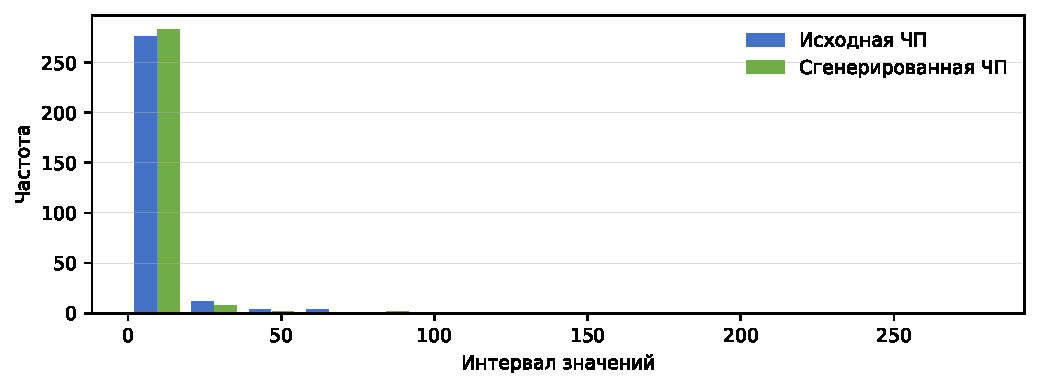
\includegraphics[width=0.93\textwidth]{figures/histogram_comparison.pdf}
\caption{Гистограммы исходной и сгенерированной последовательностей}
\end{figure}

\textbf{Вывод.} Обе последовательности имеют одинаковый качественный вид распределения: высокий первый интервал и длинный правый хвост. Частоты отдельных интервалов различаются, поскольку сравниваются две независимые реализации конечного объёма.

\subsection{Автокорреляция сгенерированной последовательности}

Коэффициенты для обоих рядов вычислены по формуле (7).

\begin{table}[H]
\centering
\caption{Коэффициенты автокорреляции}
\scriptsize
\resizebox{\textwidth}{!}{%
\begin{tabular}{lrrrrrrrrrr}
\toprule
Сдвиг & 1 & 2 & 3 & 4 & 5 & 6 & 7 & 8 & 9 & 10 \\
\midrule
Исходная ЧП & -0.041 & -0.039 & 0.034 & -0.040 & -0.045 & 0.135 & -0.029 & -0.057 & -0.027 & 0.082 \\
Сгенерированная ЧП & 0.019 & -0.032 & -0.008 & -0.035 & -0.018 & -0.016 & 0.026 & 0.015 & -0.016 & -0.010 \\
Отклонение, \% & 147.3 & 16.2 & 124.7 & 13.0 & 60.4 & 112.1 & 189.9 & 125.4 & 39.1 & 111.7 \\
\bottomrule
\end{tabular}}
\end{table}

\begin{figure}[H]
\centering
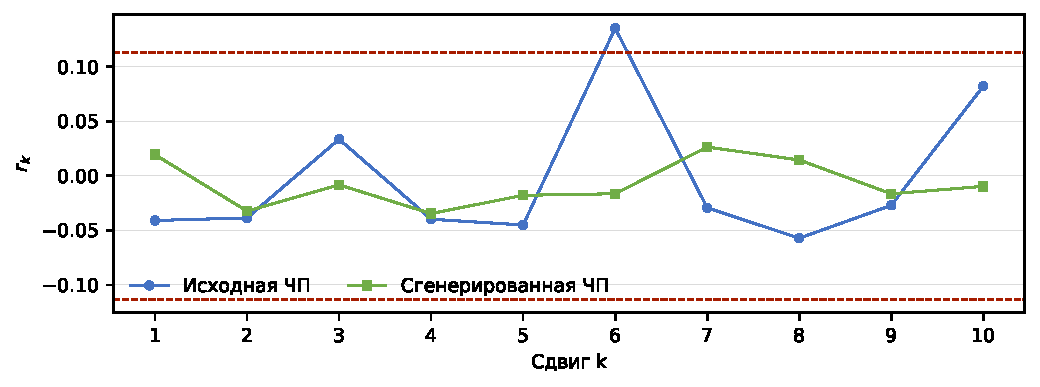
\includegraphics[width=0.93\textwidth]{figures/acf_comparison.pdf}
\caption{Сравнение автокорреляционных функций}
\end{figure}

\textbf{Вывод.} Коэффициенты сгенерированной последовательности малы и находятся внутри ориентировочных границ 95\%. Большие относительные отклонения отдельных коэффициентов не свидетельствуют о сильном различии, поскольку сами коэффициенты близки к нулю.

\subsection{Корреляция исходной и сгенерированной последовательностей}

Линейная связь между рядами оценивается коэффициентом корреляции Пирсона:
\begin{equation}
r_{xy}=\frac{\displaystyle\sum_{i=1}^{n}(x_i-\bar{x})(y_i-\bar{y})}
{\displaystyle\sqrt{\sum_{i=1}^{n}(x_i-\bar{x})^2}
\sqrt{\sum_{i=1}^{n}(y_i-\bar{y})^2}}=-0{,}0361.
\end{equation}

\textbf{Вывод.} Значение близко к нулю, поэтому существенная линейная зависимость между исходной и сгенерированной последовательностями отсутствует. Это ожидаемо для независимой контрольной реализации с тем же аппроксимирующим законом распределения.

\section{Итоговые выводы}

\begin{enumerate}
\item Для варианта 16 при $n=300$ получены $\bar{x}=8{,}0208$, $s^2=510{,}4309$, $s=22{,}5927$ и $C_v=2{,}8168$.
\item По критерию Льюнга--Бокса нет оснований отвергать отсутствие серийной зависимости.
\item Из-за $C_v>1$ для аппроксимации выбрано двухфазное гиперэкспоненциальное распределение $H_2$.
\item По первым двум моментам определены $p=0{,}940494$, $\mu_1=0{,}234515$, $\mu_2=0{,}014838$.
\item Реализован воспроизводимый генератор $H_2$ на основе LCG и обратного преобразования экспоненциального распределения.
\item При $n=300$ отклонения сгенерированного ряда составили $0{,}10\%$ по среднему и $0{,}09\%$ по дисперсии.
\item Корреляция исходной и сгенерированной последовательностей равна $-0{,}0361$, то есть существенная линейная связь отсутствует.
\end{enumerate}

\end{document}
